\documentclass[conference,compsoc
%,draft
]{IEEEtran}
%\IEEEoverridecommandlockouts

\usepackage{cite}
\usepackage{amsmath,amssymb,amsfonts}
\usepackage{algorithmic}
\usepackage{graphicx}
\usepackage{textcomp}
\usepackage{xcolor}

\usepackage{orcidlink}

\usepackage{listings}
\usepackage{xcolor}

\usepackage{balance}

\lstset{
    language=Python,
    basicstyle=\ttfamily\footnotesize,
    keywordstyle=\color{blue},
    commentstyle=\color{gray},
    stringstyle=\color{red},
    numbers=left,
    numberstyle=\tiny\color{gray},
    stepnumber=1,
    breaklines=false,
    frame=single,
    captionpos=b
}
%\usepackage{refcheck}

\def\BibTeX{{\rm B\kern-.05em{\sc i\kern-.025em b}\kern-.08emT\kern-.1667em\lower.7ex\hbox{E}\kern-.125emX}}
    
\begin{document}

\title{DEEP-SEED:\\From Scratch to Ensemble -- A Deep Learning Approach to Seedling Classification}

\author{\IEEEauthorblockN{Luca Uckermann\orcidlink{0009-0005-2957-6331}}
    \IEEEauthorblockA{\textit{Faculty of Information, Media and Electrical Engineering}\\
        \textit{Institute of Media and Imaging Technology}\\
        \textit{TH Köln -- University of Applied Sciences}\\
        Cologne, Germany\\
        luca.uckermann@th-koeln.de}
}

\maketitle

\begin{abstract}
    This paper evaluates and compares three deep learning~(DL) approaches for plant seedlings classification using a dataset consisting of \textit{4750} images of \textit{12} different plant species. Several DL approaches were considered, including a custom convolutional neural network~(CNN) trained from scratch, a pre-trained CNN ``ResNet-18'' and a pre-trained vision transformer~(ViT) ``vit-base-patch16-224'' fine-tuned for the task at hand. To address the challenges of data scarcity and class imbalance, extensive data augmentation techniques such as random rotations, flips and color jittering were employed. Results showed that transfer learning with ResNet-18 outperforms the custom model, achieving a mean F1-score~(micro-averaged) of \textbf{~0.961} on the test set. The custom CNN, still achieved a competitive F1-score of \textbf{~0.927}, demonstrating that even smaller locally trained architectures can be viable if carefully designed and thoroughly regularized. While the ViT model achieved the highest F1-score of \textbf{~0.967}, an ensemble combining the predictions of all three models outperformed the single models with a score of \textbf{~0.971}. Finally, potential improvements are outlined, including deeper architectures, synthetic image generation and interpretability measures, to further improve seedling classification performance.
\end{abstract}

\begin{IEEEkeywords}
    Machine learning, Image classification, Convolutional neural networks, Vision transformers, Transfer learning
\end{IEEEkeywords}

\section{Introduction}

This section provides an overview of the challenge, including its context, problem definition, dataset overview and key challenges.

\subsection{Context and Background}
The ``Plant Seedlings Classification'' challenge, hosted on Kaggle~\cite{plant-seedlings-classification}, presents a real-world problem central to modern agriculture: accurately identifying the species of young seedlings from digital images~\cite{MESHRAM2021100010}.

The dataset described in~\cite{DBLP:journals/corr/abs-1711-05458} contains images of approximately \textit{960} unique plants, representing \textit{12} different species~(see~Fig.~\ref{fig:sample-images}). Each image captures a seedling at different growth stages and under different conditions, reflecting the complexities found in real-world agricultural environments. These conditions include differences in lighting, background soil patterns and subtle phenotypic variations that can blur the lines between certain species.

\begin{figure}[htbp]
    \centerline{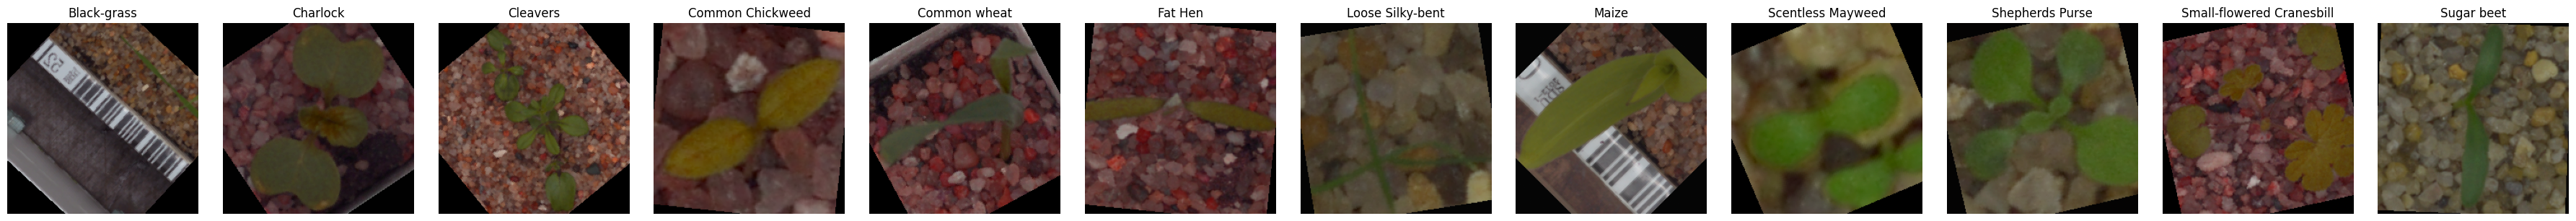
\includegraphics[width=0.9\linewidth]{../../resources/sample_images.png}}
    \caption{One sample image for each class in the dataset}
    \label{fig:sample-images}
\end{figure}

Fig.~\ref{fig:sample-images} shows one sample image for each class in the dataset, illustrating the different species. The images vary in background, lighting and growth stage, highlighting the challenges of visual similarity across species.

The evaluation metric of the competition is a mean~(micro-averaged) F1-score, which encourages balanced performance across classes~\cite{plant-seedlings-classification-evaluation}:

\begin{equation}
    \text{Precision}_{\text{micro}} = \frac{\sum_{k \in C} \mathit{TP_k}}{\sum_{k \in C} \mathit{TP_k} + \mathit{FP_k}}\label{eq:precision}
\end{equation}

\begin{equation}
    \text{Recall}_{\text{micro}} = \frac{\sum_{k \in C} \mathit{TP_k}}{\sum_{k \in C} \mathit{TP_k} + \mathit{FN_k}}\label{eq:recall}
\end{equation}

\begin{equation}
    F1_{\text{micro}} = \frac{2 \cdot \text{Precision}_{\text{micro}} \cdot \text{Recall}_{\text{micro}}}{\text{Precision}_{\text{micro}} + \text{Recall}_{\text{micro}}}\label{eq:fscore}
\end{equation}

where $TP_k$, $FP_k$ and $FN_k$ are the true positive, false positive and false negative counts for class $k$, respectively and $C$ is the set of all classes. The mean F1-score~(\ref{eq:fscore}) is a balanced measure that considers both precision~(\ref{eq:precision}) and recall~(\ref{eq:recall}) across all classes, making it a suitable evaluation metric for multi-class classification tasks.

\subsection{Problem Definition and Objectives}
The core objective of the challenge is to build an automated classification model that can take a seedling image as input and accurately predict its species. The following points summarize the task:

\begin{enumerate}
    \item \textbf{Input:} Train set of \textit{4750} images of plant seedlings.
    \item \textbf{Output:} Classification label for each image, indicating the species of each plant seedling.
    \item \textbf{Goal:} High classification performance as measured by equation~\ref{eq:fscore}.
\end{enumerate}

The challenge is to develop a model that can generalize well across different species, even when faced with variations in lighting, background and growth stages. A significant risk when dealing with deep learning~(DL) models is overfitting, especially when the dataset is relatively small~\cite[Chapter~1]{bishop2024deep}~\cite[Chapter~5]{Goodfellow-et-al-2016}. Therefore, the model must be designed to learn robust features that can generalize well to unseen data~(see~\ref{subsec:challenges}).

\subsection{Dataset Overview}
For a better understanding of the dataset, a brief overview of the class distribution and sample images is provided below:

\begin{figure}[htbp]
    \centerline{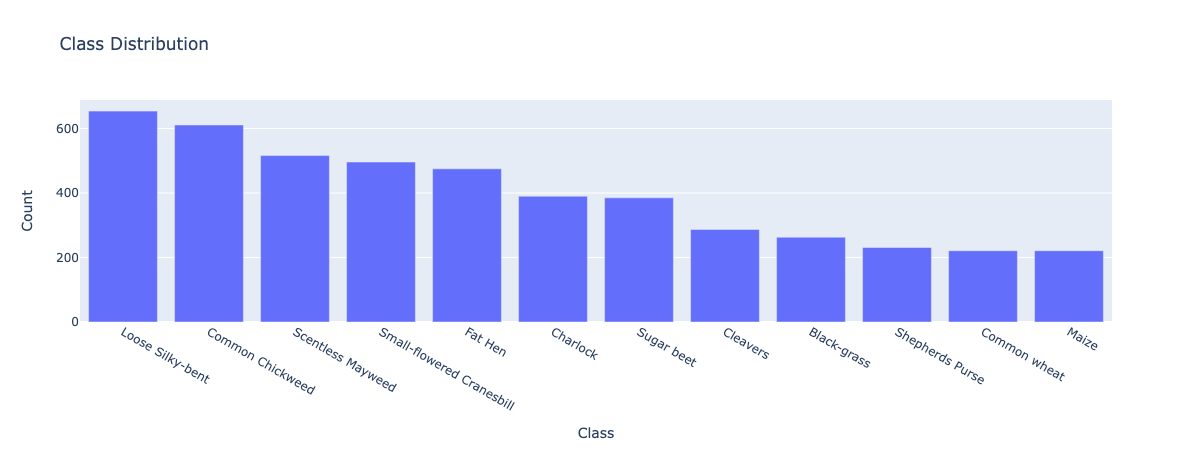
\includegraphics[width=0.9\linewidth]{../../resources/class_distribution.png}}
    \caption{Class distribution of the \textit{4750} training images}
    \label{fig:class-distribution}
\end{figure}

Fig.~\ref{fig:class-distribution} shows the distribution of classes in the train dataset, with each bar representing the number of images per class. The dataset is imbalanced, with some classes having significantly fewer samples than others. This imbalance can pose a challenge for model training, as the model may struggle to learn the features of underrepresented classes effectively. The most common classes are ``Loose Silky-bent''~(\textit{654}) and ``Common Chickweed''~(\textit{611}), while the least common classes are ``Common wheat'' and ``Maize''~(both \textit{221}).

\subsection{Key Challenges}\label{subsec:challenges}
Developing robust classification models for this task is not trivial. There are several challenges:

\begin{enumerate}
    \item \textbf{Inter-Class Similarity:} Certain seedlings can look strikingly similar, making it difficult for both humans and machines to distinguish between them.
    \item \textbf{Intra-Class Variability:} Even within a single species, seedlings can vary significantly in appearance due to differences in growth stage, lighting and background. This variability challenges models to learn consistent features that generalize well.
    \item \textbf{Data Limitations:} With approximately \textit{960} unique plants, the dataset could be considered modest for training DL models from scratch. While data augmentation can help to some extent~(see~\ref{subsec:regularization-techniques}), the relatively small dataset may still limit the complexity of models that can be effectively trained without overfitting.
    \item \textbf{Model Architecture Complexity:} Choosing the right model architecture, whether a custom convolutional neural network~(CNN)~\cite{o2015introduction} trained from scratch or a pre-trained deep CNN / Vision Transformer~(ViT)~\cite{DBLP:journals/corr/abs-2010-11929}, to learn complex visual features. Deeper models can capture more nuanced differences, but they can also be harder to train and require careful regularization to prevent overfitting~(see~\ref{subsec:regularization-techniques}).
\end{enumerate}

By clearly understanding these challenges and the broader context, model architectures can be proposed that address these difficulties. The following chapters discuss the strategies for model design, training optimization, model evaluation and analysis of results, ultimately leading to the approach that best addresses the core challenge of differentiating between plant seedling species. Finally, the conclusion summarizes the key findings and suggests potential areas for future research.
\section{Model Architecture Design}

Python and Jupyter notebooks were used to implement the models and train them on the plant seedlings dataset. The code was organized into separate notebooks for each model, allowing for easy experimentation and comparison of different architectures. Libraries such as PyTorch, Scikit-learn, NumPy and Pandas were used for data manipulation, model training and evaluation.

To achieve deterministic results and reproducibility, the random seed \textit{42} was set at the beginning of each notebook. This ensured that the same random initialization was used for each run, leading to consistent results across different experiments:

\begin{minipage}{0.9\linewidth}\begin{lstlisting}[caption={Settings to achieve deterministic results and ensure reproducibility.},label={lst:deterministic-results}]
RANDOM_SEED = 42

seed(RANDOM_SEED)
np.random.seed(RANDOM_SEED)

torch.manual_seed(RANDOM_SEED)
torch.cuda.manual_seed_all(RANDOM_SEED)

torch.backends.cudnn.deterministic = True
torch.backends.cudnn.benchmark = False
\end{lstlisting}\end{minipage}

The random seed was set for the Python, NumPy and PyTorch random number generator. Additionally, the cuDNN backend was set to deterministic mode to ensure that the results are reproducible on the GPU.

\subsection{Guessing Baseline}

As a starting point and to get familiar with the dataset and the Kaggle competition, a simple guessing baseline was implemented. The baseline assigns the most frequent class label to all test samples. This approach provided a lower bound on model performance and served as a reference point for evaluating the effectiveness of more sophisticated models. The head of the submission file is shown below:

\begin{minipage}{0.9\linewidth}\begin{lstlisting}[language={},caption={Head of guessing baseline submission file.},label={lst:guessing-baseline}]
file,species
1b490196c.png,Loose Silky-bent
85431c075.png,Loose Silky-bent
506347cfe.png,Loose Silky-bent
7f46a71db.png,Loose Silky-bent
668c1007c.png,Loose Silky-bent
...
\end{lstlisting}\end{minipage}

In this case, all \textit{794} test samples were assigned the class label ``Loose Silky-bent'', which is the most frequent class in the training dataset. The F1-score of this baseline is \textbf{0.14105}.

\subsection{Custom CNN}

The custom CNN architecture was designed to capture features relevant to seedling classification, while being lightweight enough to be effectively trained locally on the given dataset. The model consists of a series of convolutional and pooling layers followed by fully connected layers to learn features hierarchically and make the final class prediction.

\begin{figure}[htbp]
    \centerline{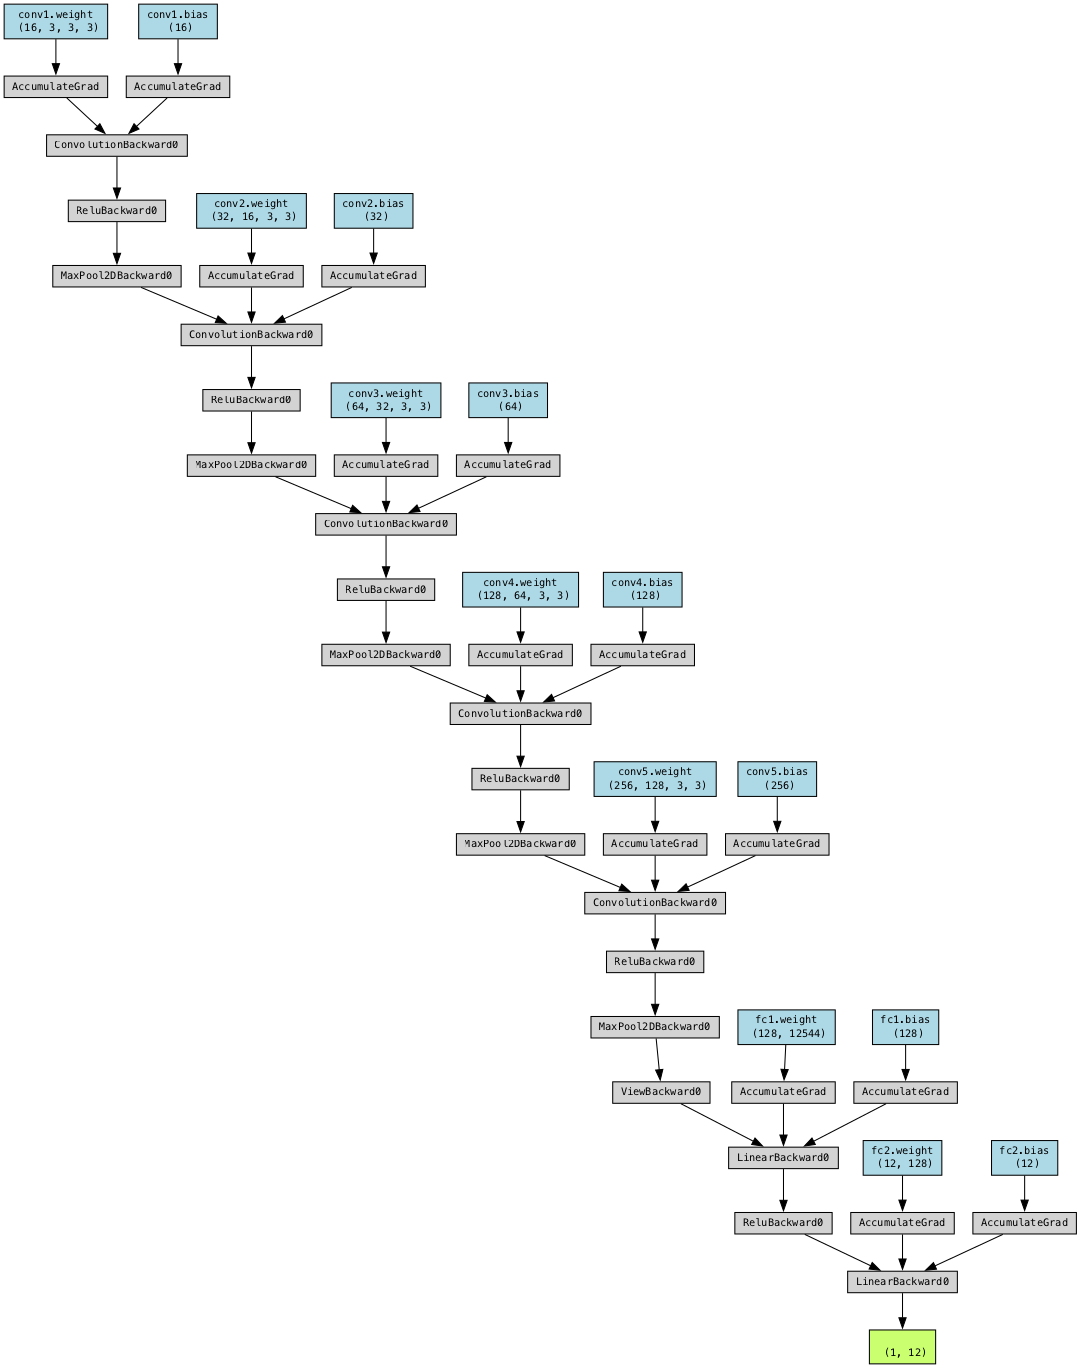
\includegraphics[width=0.9\linewidth]{../../resources/custom_cnn/architecture.png}}
    \caption{Custom CNN architecture, consisting of convolutional and pooling layers followed by fully connected layers.}
    \label{fig:custom-cnn-architecture}
\end{figure}

As shown in Fig.~\ref{fig:custom-cnn-architecture}, the network begins with a series of convolutional layers, with the number of filters gradually increasing from \textit{16} to \textit{256}. These convolutional layers, each followed by a Rectified Linear Unit~(ReLU) activation, extract spatial features such as edges, textures and patterns from the images. To reduce spatial dimensions and computational complexity, max-pooling layers are applied after each convolutional block to focus on the most salient features.

After the convolutional and pooling stages, the feature maps are flattened into a 1D vector that serves as the input to the fully connected layers. The first fully connected layer has \textit{128} neurons and captures high-level abstract features, while the final fully connected layer maps these features to the \textit{12} target classes, producing the class probabilities.

The final custom CNN model has approximately \textit{2 million} parameters, making it lightweight and computationally efficient compared to the following architectures. The model architecture is designed to capture relevant features for seedling classification while being suitable for training on a moderate-sized dataset.

\subsection{Pre-trained CNN}

As an alternative to training a custom CNN from scratch, a pre-trained CNN can be used to leverage learned features from a large dataset. The pre-trained model ResNet-18~\cite{DBLP:journals/corr/HeZRS15} was used as a feature extractor, where the final classification layer was replaced with a new fully connected layer to predict the \textit{12} plant seedling classes:

\begin{minipage}{0.9\linewidth}\begin{lstlisting}[caption={Replacing the final classification layer of a pre-trained ResNet-18 model.},label={lst:pre-trained-cnn}]
from torchvision import models
from torch.nn import Linear

model = models.resnet18(
    weights=models.ResNet18_Weights.DEFAULT
)
model.fc = Linear(
    in_features=model.fc.in_features,
    out_features=len(dataset.classes),
)
\end{lstlisting}\end{minipage}

The \texttt{ResNet18} model has been pre-trained on the ImageNet dataset~\cite{5206848ImageNet} and has shown strong performance on a variety of computer vision tasks~\cite{DBLP:journals/corr/HeZRS15}. By using a pre-trained model, the network can leverage the learned features from ImageNet to improve performance on the plant seedlings dataset. The final classification layer was replaced to adapt the model to the specific classification task.

This pre-trained CNN model has approximately \textit{11 million} parameters, making it deeper than the custom CNN. However, fine-tuning the weights allow the model to learn more complex features and hopefully achieve better performance on the plant seedlings dataset.

\subsection{Pre-trained ViT}

Another approach is to use a ViT as the backbone architecture. The ViT model has been pre-trained on \mbox{ImageNet-21k}~\cite{ridnik2021imagenet}~(including plants/crops) and then fine-tuned~\cite{steiner2021train} on the plant seedlings dataset. The final classification head was replaced with a new linear layer to predict the \textit{12} plant seedling classes:

\begin{minipage}{0.9\linewidth}\begin{lstlisting}[caption={Replacing the final classification layer of a pre-trained ViT model.},label={lst:pre-trained-vit}]
import timm
import torch

model = timm.create_model(
    "vit_base_patch16_224",
    pretrained=True,
    num_classes=num_classes
)
model.head = torch.nn.Linear(
    model.head.in_features,
    num_classes
)
\end{lstlisting}\end{minipage}

Instead of fine-tuning the entire model, the pre-trained weights of the \texttt{vit\_base\_patch16\_224} model~\cite{Wightman_PyTorch_Image_Models} were frozen and only the classification head was trained on the plant seedlings dataset. Transfer learning leverages the powerful feature extraction capabilities of the pre-trained model while adapting the final layer to the specific classification task~\cite[Chapter~6]{bishop2024deep}. Furthermore the computational cost is reduced compared to training the entire model from scratch or fine-tuning all layers:

\begin{minipage}{0.9\linewidth}\begin{lstlisting}[caption={Freezing the pre-trained ViT backbone and training only the classification head.},label={lst:freeze-vit-backbone}]
for param in model.parameters():
    param.requires_grad = False

for param in model.head.parameters():
    param.requires_grad = True
\end{lstlisting}\end{minipage}

The ViT model has approximately \textit{86 million} parameters, but only \textit{9,228} of these are adapted in the experiments. This makes the model computationally efficient, while still benefiting from the powerful feature extraction capabilities of the pre-trained ViT model.

\subsection{Ensemble}

Several challenges have shown that an ensemble of models can often outperform individual models, especially when inference time is not a primary concern~\cite{Stallkamp2012,DBLP:journals/corr/HeZRS15}. A final ensemble was created by combining the predictions of all three models (custom CNN, pre-trained CNN, pre-trained ViT) using a weighted average. The weights were determined based on the performance of each model on the test set:

\begin{minipage}{0.9\linewidth}\begin{lstlisting}[caption={Ensemble predictions using a weighted average.},label={lst:ensemble}]
import torch.nn.functional as F

model_custom_cnn.eval()
model_resnet.eval()
model_vit.eval()

w_custom_cnn = 0.25
w_resnet = 0.25
w_vit = 1 - w_custom_cnn - w_resnet

...

probs_custom_cnn = (
    F.softmax(model_custom_cnn(images), dim=1)
)
probs_resnet = (
    F.softmax(model_resnet(images), dim=1)
)
probs_vit = (
    F.softmax(model_vit(images), dim=1)
)

probs_ensemble = (
    w_custom_cnn * probs_custom_cnn +
        w_resnet * probs_resnet +
            w_vit * probs_vit
)

_, preds = torch.max(probs_ensemble, 1)
\end{lstlisting}\end{minipage}

The ensemble combines the strengths of each individual model to improve overall performance and robustness. By averaging the predictions of multiple models, the ensemble can reduce the impact of individual model weaknesses and provide more reliable predictions (\textit{wisdom of the crowd}~\cite[Chapter~7]{geronoctober2022hands}). As the ViT model achieved the highest performance on the test set, it is assigned the highest weight in the ensemble (\textit{0.5}), while the custom CNN and ResNet models are assigned equal weights (both \textit{0.25}).

\subsection{Summary}

\begin{table}[htbp]
    \caption{Model parameters and size of the custom CNN, pre-trained CNN and pre-trained ViT.}
    \begin{center}
        \resizebox{0.9\linewidth}{!}{
            \begin{tabular}{|c|c|c|c|}
                \hline
                \textbf{Model}  & \textbf{Total Params} & \textbf{Trainable params} & \textbf{Total Size (MB)} \\
                \hline
                Custom CNN      & 1,999,916             & 1,999,916                 & 34.91                    \\
                \hline
                Pre-trained CNN & 11,182,668            & 11,182,668                & 106.02                   \\
                \hline
                Pre-trained ViT & 85,655,820            & 9,228                     & 806.35                   \\
                \hline
            \end{tabular}
            \label{tab:parameters}
        }
    \end{center}
\end{table}

Table~\ref{tab:parameters} shows the total number of parameters and the size of each model. The custom CNN has the smallest number of parameters and size, making it lightweight and computationally efficient. The pre-trained CNN has a larger number of parameters, while the pre-trained ViT has the largest, but only a small fraction of them are trainable during the experiments. This allows for efficient training while still benefiting from the powerful feature extraction capabilities of the pre-trained model.
\section{Training Optimization Strategies}

This section describes the training algorithms, learning rate schedules and regularization techniques used to improve model generalization and prevent overfitting.

\subsection{Training Algorithms and Optimizers}\label{subsec:training-algorithms-optimizers}

All models were trained using the Adam optimizer~\cite{kingma2017adammethodstochasticoptimization} with a learning rate of \textit{0.001}. The Adam optimizer is a popular choice for training deep neural networks due to its adaptive learning rate mechanism and momentum-based updates. A weight decay of \textit{1e-4} was applied to regularize the model and prevent overfitting~(see~\ref{subsec:regularization-techniques}).

\subsection{Learning Rate Schedules}

To adjust the learning rate during training, a learning rate scheduler was used to reduce the learning rate by a factor of \textit{0.5} if the validation loss did not improve for \textit{2} epochs. This technique helps the model converge more effectively by gradually reducing the learning rate as it approaches a local minimum.

\subsection{Regularization Techniques}\label{subsec:regularization-techniques}

To prevent overfitting and improve generalization, several regularization techniques were applied during training:

\begin{itemize}
    \item \textbf{Weight Decay:} L2 regularization with a weight decay of \textit{1e-4} was applied to the optimizer to penalize large weights (see~\ref{subsec:training-algorithms-optimizers}).
    \item \textbf{Dropout:} A dropout layer with a dropout probability of \textit{0.5} was added after the fully connected layer to regularize the model and prevent co-adaptation of neurons.
    \item \textbf{Data Augmentation:} Various data augmentation techniques such as random rotations, flips and color jittering were applied to the training images to increase the diversity of the training set and improve the robustness of the model~(see Fig.~\ref{fig:data-augmentation}).
\end{itemize}

\begin{figure}[htbp]
    \centerline{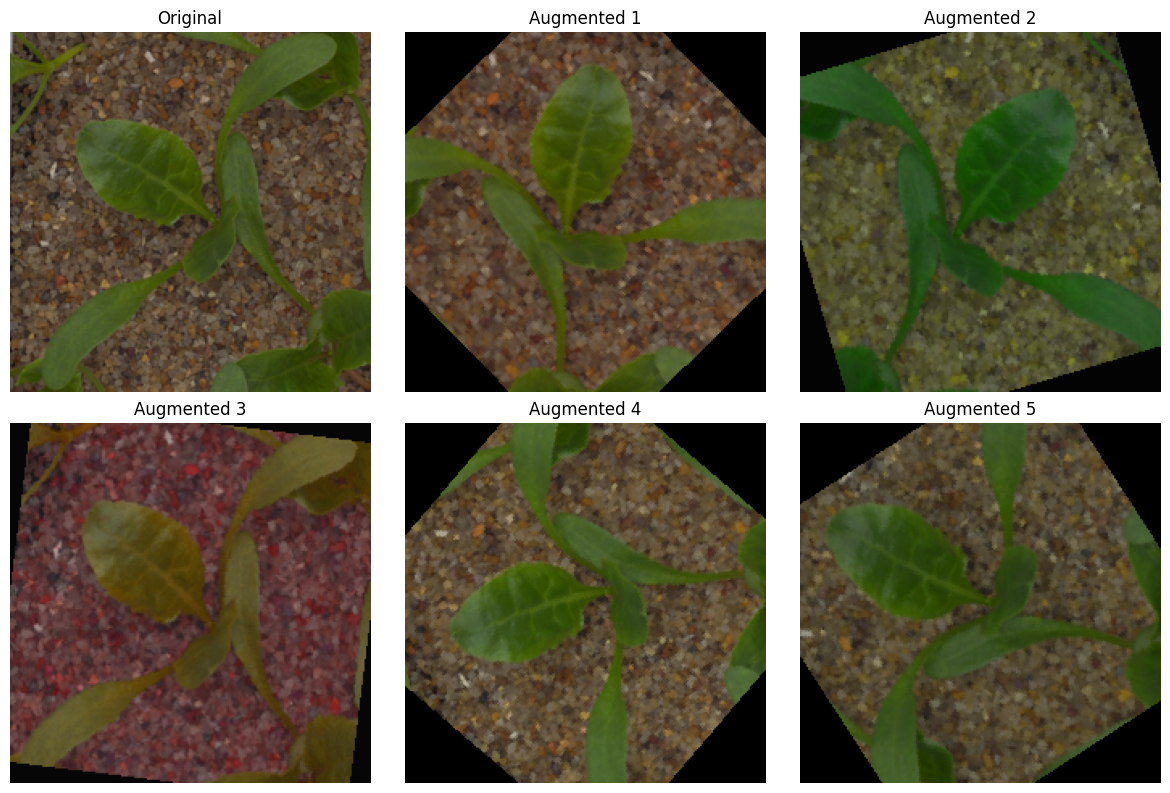
\includegraphics[width=0.9\linewidth]{../../resources/data_augmentation.png}}
    \caption{Original image~(top left) and five augmented versions.}
    \label{fig:data-augmentation}
\end{figure}

Fig.~\ref{fig:data-augmentation} shows one original image of the given dataset and five augmented versions. The augmentations include random rotations, flips and color jittering, which help the models learn more robust features and improve generalization to unseen data. During training those augmentations were applied randomly to each image, while the original images were used for validation. This approach allowed the model to learn from a more diverse set of training samples without introducing bias in the validation process.
\section{Model Evaluation and Validation}

\subsection{Validation Framework}

To evaluate the performance of the models during training, the dataset was split into training and validation sets using a stratified split with a ratio of \textbf{80:20}. The validation set was used to monitor performance during training and prevent overfitting.

\begin{minipage}{0.9\linewidth}\begin{lstlisting}[caption={Stratified split of the dataset into training and validation sets.},label={lst-train-vald-split}]
from sklearn.model_selection import train_test_split
from torch.utils.data import Subset

labels = [label for _, label in dataset.samples]
train_indices, val_indices = train_test_split(
    range(len(dataset)),
    test_size=0.2,
    stratify=labels,
    random_state=RANDOM_SEED
)

train_dataset = Subset(dataset, train_indices)
val_dataset = Subset(dataset, val_indices)
\end{lstlisting}\end{minipage}

Since the dataset is imbalanced, a stratified split was used to ensure that the class distribution in the training and validation sets is similar. This prevents the model from overfitting the training set and ensures that it generalizes well to unseen data.

This split results in a training set of \textbf{3800} and a validation set of \textbf{950} samples (see~Fig.~\ref{fig:train-vald-split}).

\begin{figure}[htbp]
    \centerline{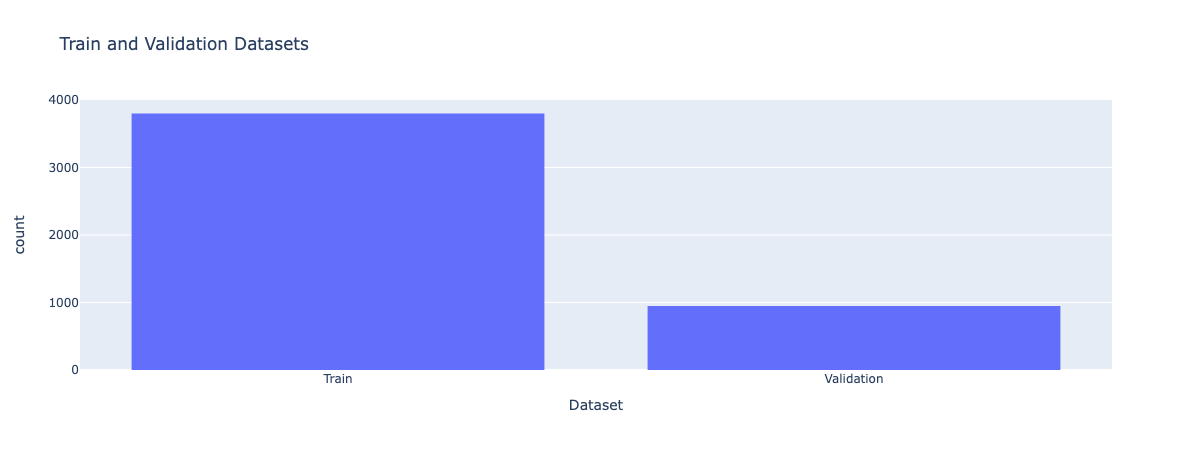
\includegraphics[width=0.9\linewidth]{../../resources/train_vald_split.png}}
    \caption{Training and Validation Set Sizes}
    \label{fig:train-vald-split}
\end{figure}

Since there are no labels for the test set, the validation set serves as a proxy to evaluate the performance of the model on unseen data. Validation loss and accuracy were monitored during training to assess the convergence and generalization capabilities of the models:

\begin{figure}[htbp]
    \centerline{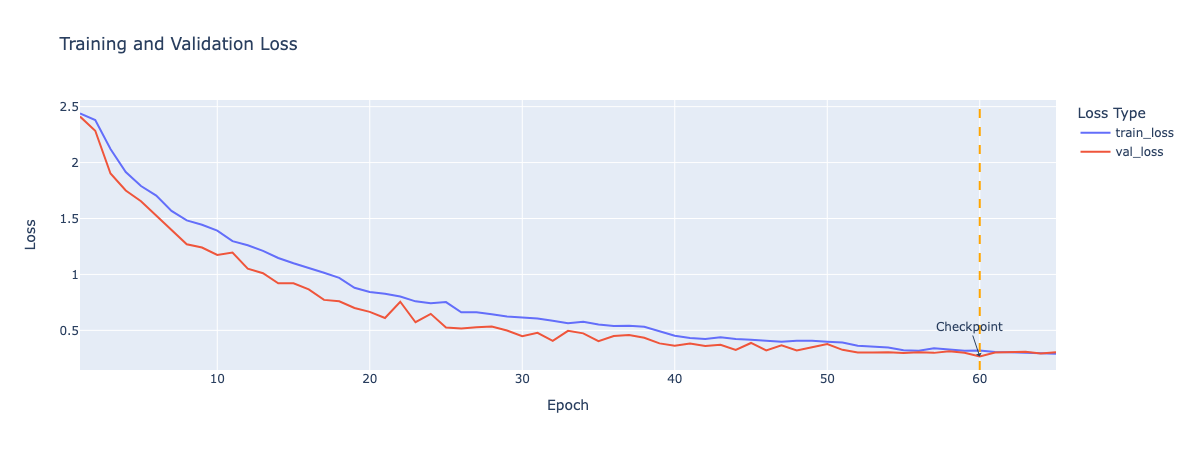
\includegraphics[width=0.9\linewidth]{../../resources/custom_cnn/loss.png}}
    \caption{Training and Validation Loss (custom CNN)}
    \label{fig:loss-custom-cnn}
\end{figure}

\begin{figure}[htbp]
    \centerline{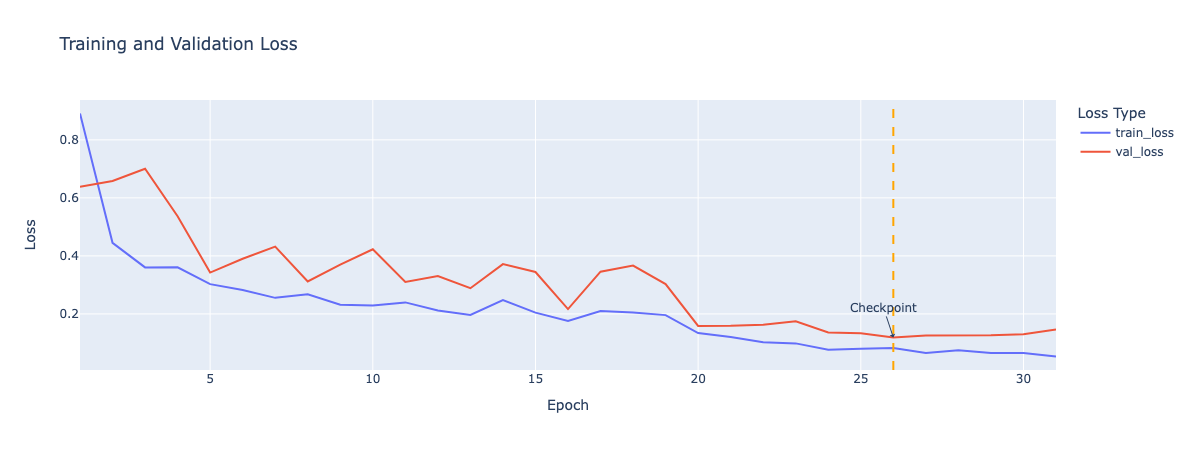
\includegraphics[width=0.9\linewidth]{../../resources/resnet/loss.png}}
    \caption{Training and Validation Loss (pre-trained CNN)}
    \label{fig:loss-pretrained-cnn}
\end{figure}

\begin{figure}[htbp]
    \centerline{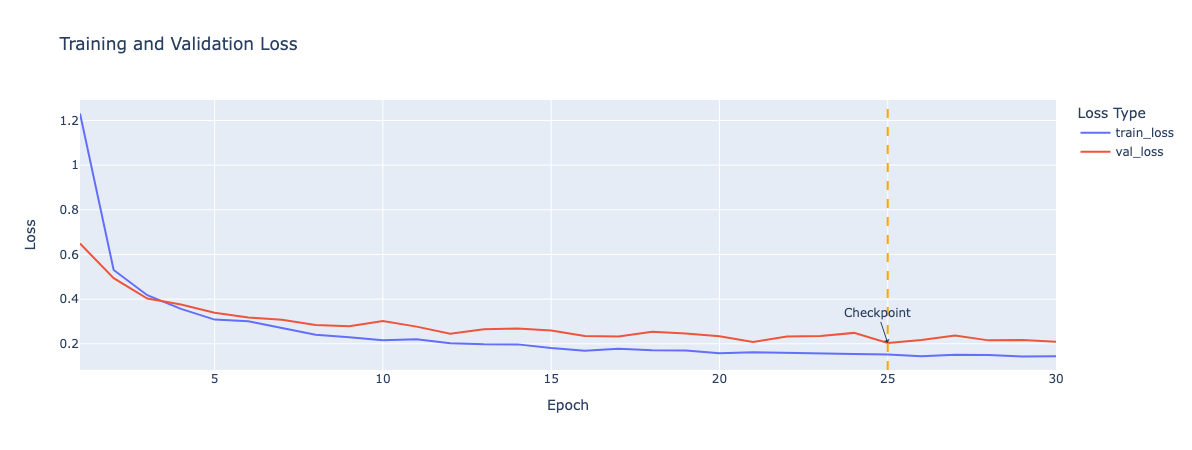
\includegraphics[width=0.9\linewidth]{../../resources/vit/loss.png}}
    \caption{Training and Validation Loss (pre-trained ViT)}
    \label{fig:loss-pretrained-vit}
\end{figure}

Fig.~\ref{fig:loss-custom-cnn}, Fig.~\ref{fig:loss-pretrained-cnn} and Fig.~\ref{fig:loss-pretrained-vit} show the training and validation loss curves for the custom CNN, pre-trained CNN and pre-trained ViT models, respectively. Each curve illustrates the learning dynamics of the model over successive epochs.

The custom CNN demonstrates a gradual reduction in both training and validation loss, converging steadily around epoch \textbf{60}. This indicates effective learning without significant overfitting, as the training and validation loss curves remain closely aligned. One could argue that the model could benefit from increased complexity and further training to improve performance.

The pre-trained CNN shows faster convergence, with training and validation loss stabilizing around epoch \textbf{25}. This faster convergence reflects the advantages of transfer learning, as the model uses pre-trained weights for feature extraction. Similarly, the pre-trained ViT, which also converges rapidly within \textbf{25} epochs, demonstrates the effectiveness of using pre-trained models for this classification task. However the gap between training and validation loss suggests that the model could benefit from additional regularization or fine-tuning to improve generalization. In particular, the pre-trained CNN begins to clearly overfit the data after epoch \textbf{30}.

The inclusion of a checkpoint in each figure highlights the point at which the model achieved the lowest validation loss, signaling optimal performance and serving as a reference for saving the best model state. The loaded checkpoints are at epoch *60*, *26* and *25* for the custom CNN, pre-trained CNN and pre-trained ViT, respectively.

\subsection{Performance Metrics}

In addition to losses, validation accuracy is tracked during training to monitor performance of the models. Accuracy is calculated as the ratio of correctly predicted samples to the total number of samples in the validation set:

\begin{equation}
    \text{Accuracy} = \frac{\text{Number of Correct Predictions}}{\text{Total Number of Samples}}\label{eq:accuracy}
\end{equation}

The accuracy (\ref{eq:accuracy}) provides a simple and intuitive measure of performance on the validation set.

\begin{figure}[htbp]
    \centerline{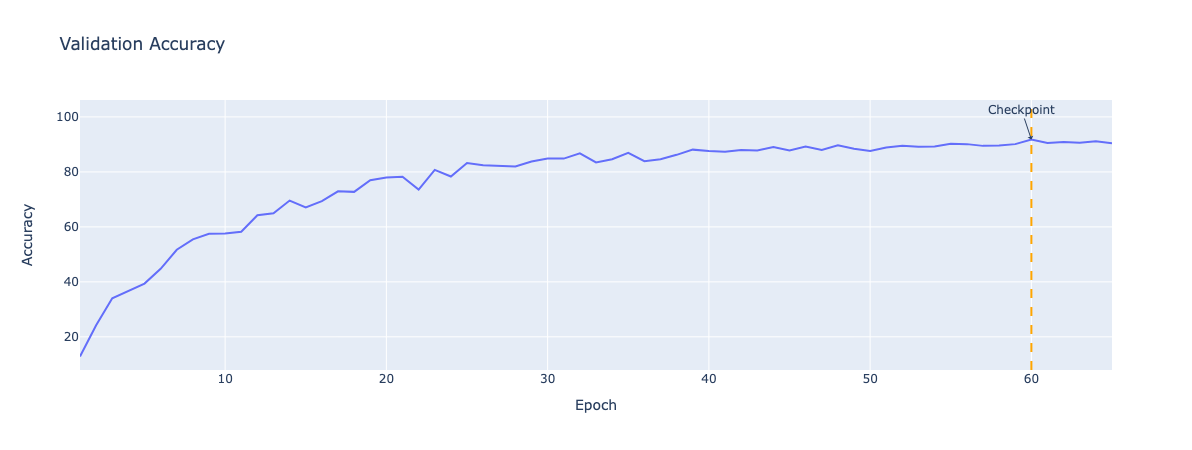
\includegraphics[width=0.9\linewidth]{../../resources/custom_cnn/accuracy.png}}
    \caption{Validation Accuracy (custom CNN)}
    \label{fig:accuracy-custom-cnn}
\end{figure}

\begin{figure}[htbp]
    \centerline{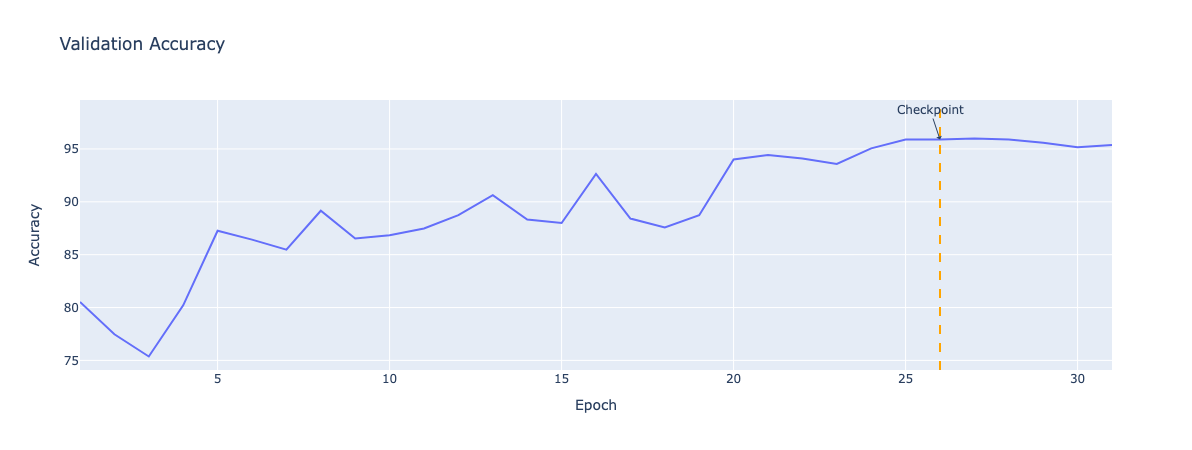
\includegraphics[width=0.9\linewidth]{../../resources/resnet/accuracy.png}}
    \caption{Validation Accuracy (pre-trained CNN)}
    \label{fig:accuracy-pretrained-cnn}
\end{figure}

\begin{figure}[htbp]
    \centerline{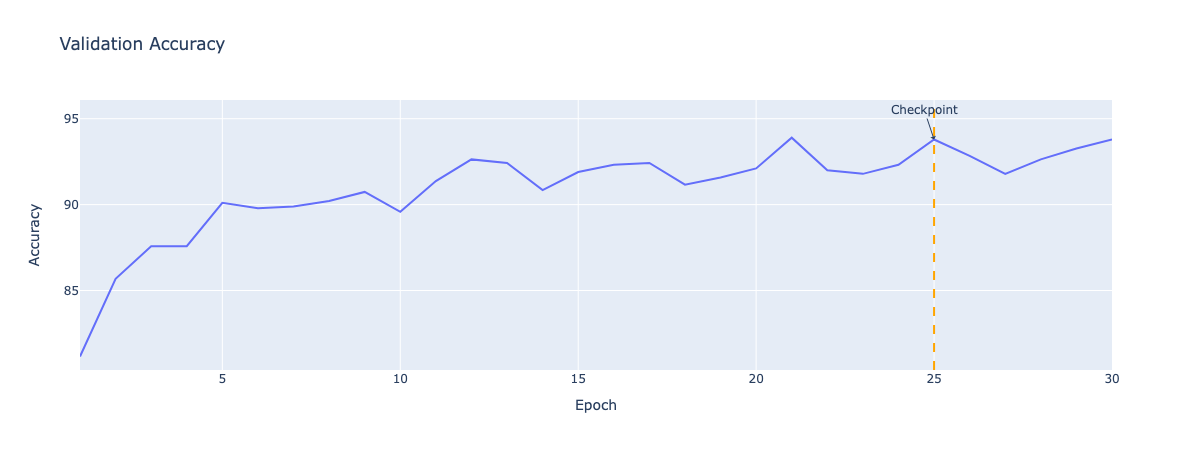
\includegraphics[width=0.9\linewidth]{../../resources/vit/accuracy.png}}
    \caption{Validation Accuracy (pre-trained ViT)}
    \label{fig:accuracy-pretrained-vit}
\end{figure}

Similar to the loss curves, Fig.~\ref{fig:accuracy-custom-cnn}, Fig.~\ref{fig:accuracy-pretrained-cnn} and Fig.~\ref{fig:accuracy-pretrained-vit} show the validation accuracy of the custom CNN, pre-trained CNN and pre-trained ViT models, respectively. The accuracy curves provide insight into the ability of the model to correctly classify the validation samples over successive epochs. The figures highlight the information from the loss curves, showing that the pre-trained models converge faster and achieve higher accuracy compared to the custom CNN. But again, the custom CNN shows a steady and smooth increase in accuracy over time, indicating that the model continues to learn and improve its performance. The selected checkpoints are the same as for the loss curves, indicating the load state of the model with the lowest validation loss, which also corresponds to high accuracy.
\section{Results and Analysis}

\subsection{Quantitative Results}

The final results for each model are presented below:

\begin{table}[htbp]
    \caption{Quantitative results of the models on the train, validation and test set.}
    \begin{center}
        \resizebox{0.9\linewidth}{!}{
            \begin{tabular}{|c|c|c|c|c|c|}
                \hline
                \textbf{Model}    & \textbf{Train Loss} & \textbf{Val Loss} & \textbf{Val Accuracy} & \textbf{Test F1-Score} & \textbf{Epochs} \\
                \hline
                Guessing Baseline & -                   & -                 & -                     & 0.14105                & -               \\
                \hline
                Custom CNN        & 0.2897              & 0.3034            & 0.9042                & 0.92695                & 64              \\
                \hline
                Pre-trained CNN   & \textbf{0.0532}     & \textbf{0.1467}   & \textbf{0.9537}       & 0.96095                & 30              \\
                \hline
                Pre-trained ViT   & 0.1438              & 0.2089            & 0.9379                & \textbf{0.96725}       & 29              \\
                \hline
                \textbf{Ensemble} & -                   & -                 & -                     & \textbf{0.97103}       & -               \\
                \hline
            \end{tabular}
            \label{tab:results}
        }
    \end{center}
\end{table}

Table~\ref{tab:results} shows the performance of each model on the validation and the test set. The \textit{custom CNN} achieved a validation accuracy of \textbf{90.42\%} and a test F1-score of \textbf{0.92695}. The \textit{pre-trained CNN}~(ResNet-18) outperformed the custom CNN with a validation accuracy of \textbf{95.37\%} and a test F1-score of \textbf{0.96095}. The \textit{pre-trained ViT}~(vit-base-patch16-224) achieved a validation accuracy of \textbf{93.79\%} and a test F1-score of \textbf{0.96725}. The \textit{ensemble}, which combines the predictions of all three models, achieved the highest test F1-score of \textbf{0.97103}. Since the \textit{guessing baseline} and the \textit{ensemble} are not trained models, the training and validation losses are not applicable.

\subsection{Qualitative Results}

Since the labels for the test set are not available, the qualitative results are based on the validation set to get an idea of the performance of the models. The confusion matrices of the custom CNN, pre-trained CNN and ViT models on the validation set are shown below:

\begin{figure}[htbp]
    \centerline{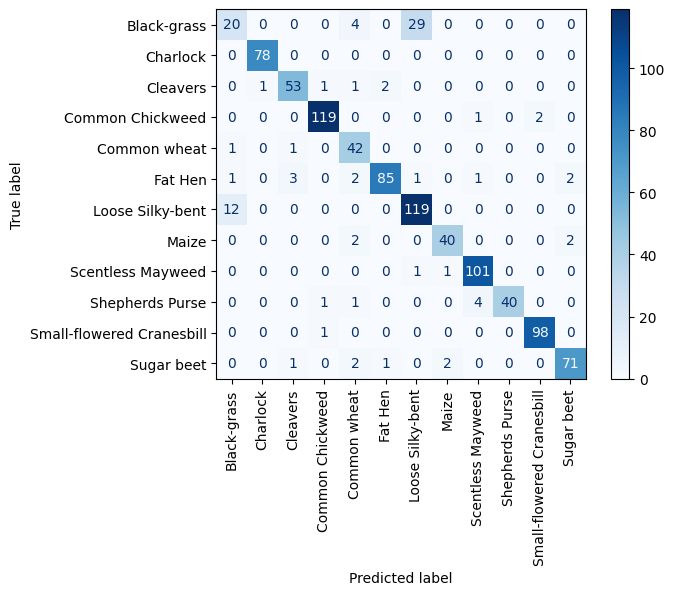
\includegraphics[width=0.9\linewidth]{../../resources/custom_cnn/confusion.png}}
    \caption{Confusion matrix~(custom CNN)}
    \label{fig:confusion-matrix-custom-cnn}
\end{figure}

Fig.~\ref{fig:confusion-matrix-custom-cnn} shows the confusion matrix of the custom CNN on the validation set. The rows represent the true classes, while the columns represent the predicted classes. The diagonal elements represent the number of correct predictions for each class, while the off-diagonal elements represent the misclassifications. While there are some misclassifications without a clear pattern, the model clearly struggles to distinguish between ``Loose Silky-bent'' and ``Black-grass''.

\begin{figure}[htbp]
    \centerline{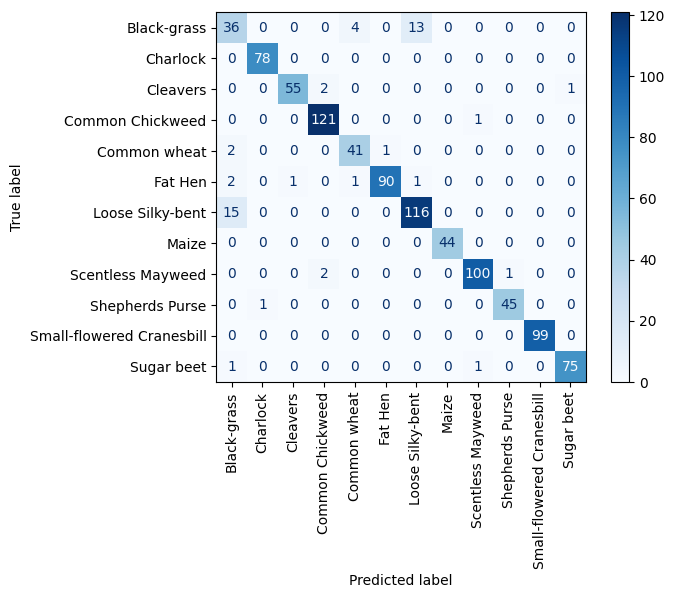
\includegraphics[width=0.9\linewidth]{../../resources/resnet/confusion.png}}
    \caption{Confusion matrix~(pre-trained CNN)}
    \label{fig:confusion-matrix-pretrained-cnn}
\end{figure}

Similar to the custom CNN, Fig.~\ref{fig:confusion-matrix-pretrained-cnn} shows the confusion matrix of the pre-trained CNN on the validation set. The model shows the same difficulty in distinguishing between ``Loose Silky-bent'' and ``Black-grass''.

\begin{figure}[htbp]
    \centerline{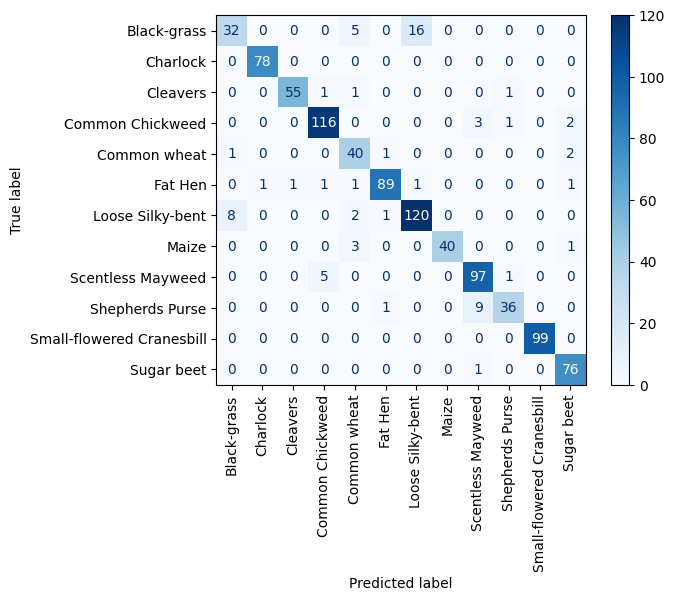
\includegraphics[width=0.9\linewidth]{../../resources/vit/confusion.png}}
    \caption{Confusion matrix~(pre-trained ViT)}
    \label{fig:confusion-matrix-pretrained-vit}
\end{figure}

Although the pre-trained ViT model takes a different approach, Fig.~\ref{fig:confusion-matrix-pretrained-vit} shows that it also struggles with the same pair of classes ``Loose Silky-bent'' and ``Black-grass''.

\subsection{Comparative Analysis}

The results show that the ensemble model outperforms the individual models, achieving the highest test F1-score of \textbf{0.97103}. The pre-trained ViT model achieved the highest individual test F1-score of \textbf{0.96725}, followed by the pre-trained CNN with a test F1-score of \textbf{0.96095}. The custom CNN achieved a test F1-score of \textbf{0.92695}, demonstrating competitive performance despite being trained from scratch.

Since real-time inference is not required for this task, the computational cost of the models is not a primary concern. However, the custom CNN is the lightest model with approximately \textit{2 million} parameters, making it computationally efficient. The pre-trained CNN has approximately \textit{11 million} parameters, while the pre-trained ViT has approximately \textit{86 million} parameters, making it the most computationally expensive model.

\subsection{Interpretability Measures}

The Pytorch-Grad-CAM library~\cite{jacobgilpytorchcam} by Jacob Gildenblat was used to generate class activation maps~(CAMs) for the custom CNN, pre-trained CNN and ViT models. CAMs provide insight into the regions of the image that the model focuses on when making predictions and can help explain the decision-making process of the model. The library was installed with the following command:

\begin{minipage}{0.9\linewidth}\begin{lstlisting}[language={},caption={Install Pytorch-Grad-CAM library.},label={lst:install-grad-cam}]
pip install grad-cam
\end{lstlisting}\end{minipage}

The simplified code snippet below shows how to generate CAMs for a given image using the custom CNN model:

\begin{minipage}{0.9\linewidth}\begin{lstlisting}[caption={Generate CAMs using Pytorch-Grad-CAM.},label={lst:grad-cam}]
from pytorch_grad_cam import GradCAM
from pytorch_grad_cam.utils.image
    import show_cam_on_image
from pytorch_grad_cam.utils.model_targets
    import ClassifierOutputTarget

with GradCAM(
        model=model,
        target_layers=target_layers,
     ) as cam:
    gs_cam = cam(
                input_tensor
                    =image.unsqueeze(0),
                targets
                    =targets,
             )
    gs_cam = gs_cam[0, :]
    visualization = show_cam_on_image(
                        rgb_img,
                        gs_cam,
                        use_rgb=True,
                    )
\end{lstlisting}\end{minipage}

\begin{figure}[htbp]
    \centerline{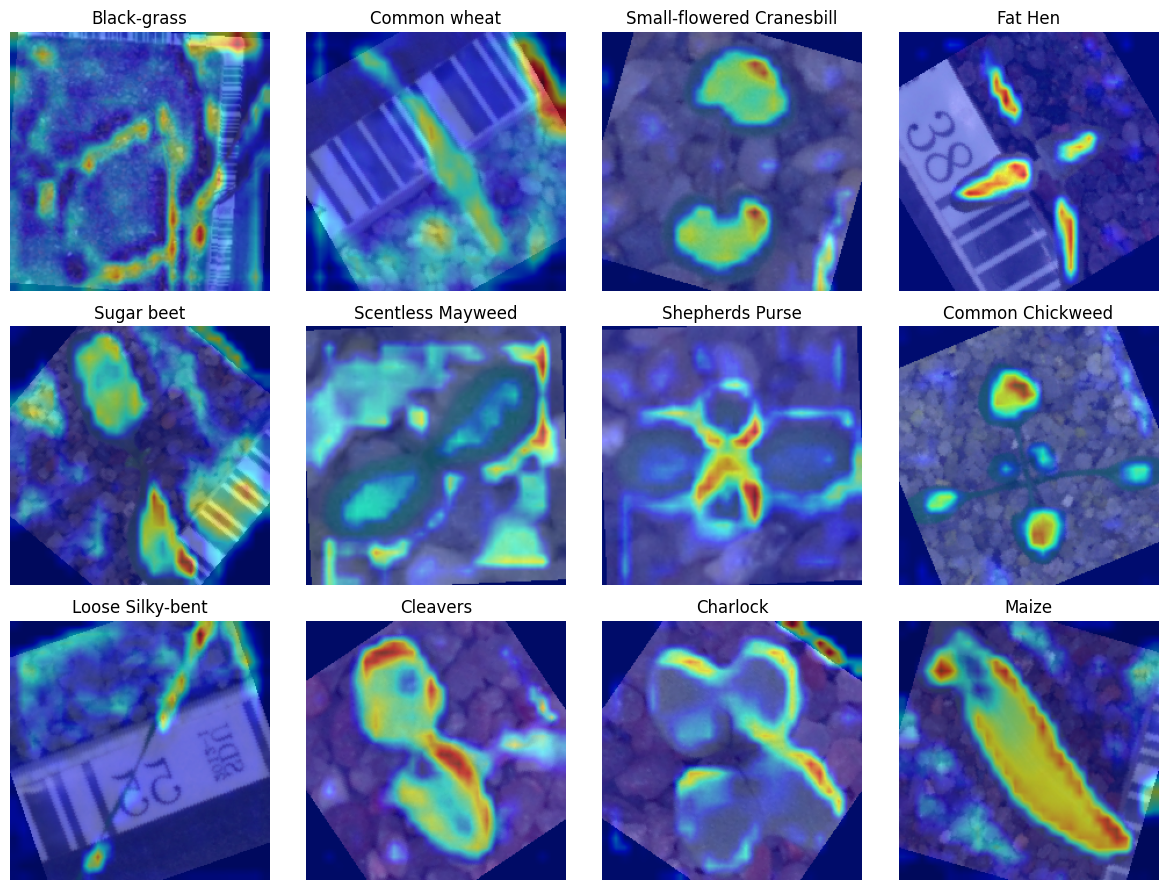
\includegraphics[width=0.9\linewidth]{../../resources/custom_cnn/grad_cam.png}}
    \caption{Grad-CAM~(custom CNN)}
    \label{fig:grad-cam-custom-cnn}
\end{figure}

\begin{figure}[htbp]
    \centerline{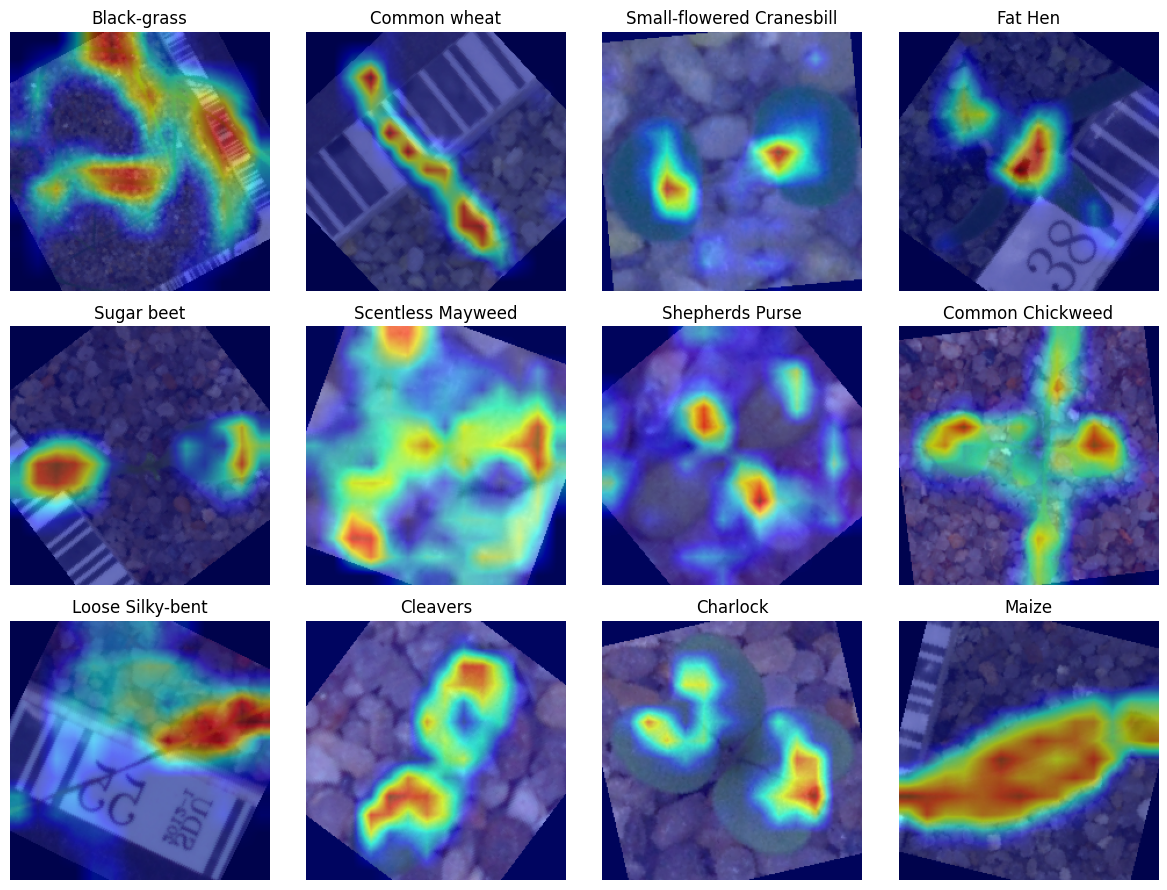
\includegraphics[width=0.9\linewidth]{../../resources/resnet/grad_cam.png}}
    \caption{Grad-CAM~(pre-trained CNN)}
    \label{fig:grad-cam-pretrained-cnn}
\end{figure}

\begin{figure}[htbp]
    \centerline{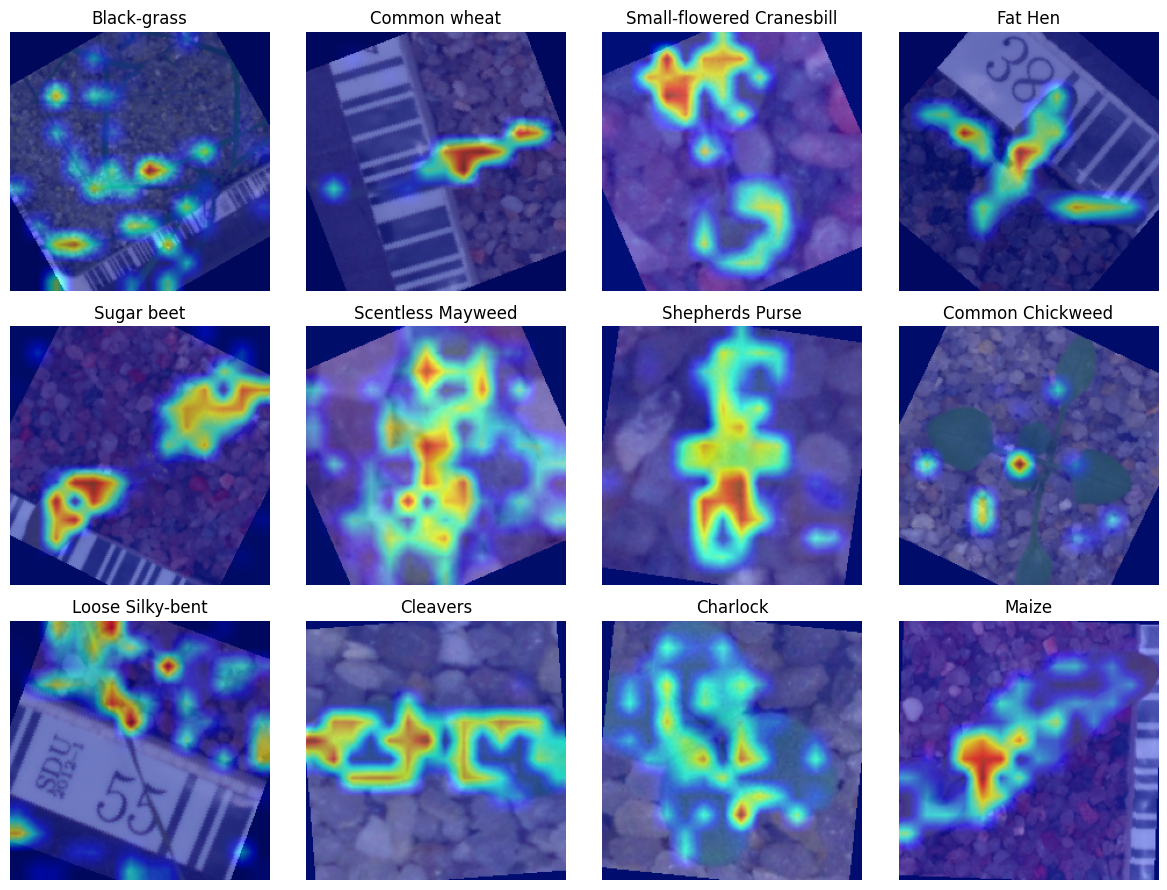
\includegraphics[width=0.9\linewidth]{../../resources/vit/grad_cam.png}}
    \caption{Grad-CAM~(pre-trained ViT)}
    \label{fig:grad-cam-pretrained-vit}
\end{figure}

The Fig.~\ref{fig:grad-cam-custom-cnn}, Fig.~\ref{fig:grad-cam-pretrained-cnn} and Fig.~\ref{fig:grad-cam-pretrained-vit} show the Grad-CAM visualizations for the last two layers of the custom CNN, pre-trained CNN and ViT models. The visualizations highlight the regions of the image that the model focuses on when making predictions. The Grad-CAM visualizations provide insight into the decision-making process of the models and help to interpret their predictions.

For some classes, such as ``Small-flowered Cranesbill'', ``Fat Hen'', ``Common Chickweed'', ``Cleavers'' and ``Maize'', the custom CNN clearly focuses on parts of the plants that a human would use to distinguish between the classes. For these species, the focus is on the leaves. For classes like ``Black-grass'', ``Common wheat'', ``Sugar beet'', ``Scentsless Mayweed'' and ``Loose Silky-bent'' the CNN focuses on what appears to be the soil or the background. One could argue that the model has difficulty distiguishing between the plants and the background and focuses on \textit{noise} in the images.

In comparison, both pre-trained architectures, the CNN and the ViT, focus more on the plants themselves. But even for ``Black-grass'', ``Scentsless Mayweed'' and ``Loose Silky-bent'' the models do not seem to focus on the plants alone. The visualizations of the areas of interest are smoother for the CNN compared to the ViT, which looks more \textit{blocky}. This is due to the different architectures and the way the models process the images as the ViT divides the image into patches and processes them separately, therefore the patches are more visible in the Grad-CAM visualizations for the ViT. For a human observer the Grad-CAM visualizations can help understand how the models make their predictions and what features they focus on, the pre-trained CNN seems to produce the most reasonable visualizations and focus on understandable features.
\section{Conclusion and Lessons Learned}

\subsection{Key Takeaways}

In this project, several strategies were explored to classify plant seedlings into \textit{12} different species, with the overall goal of achieving robust performance as measured by the mean~(micro-averaged) F1-score. Data augmentation played a central role in preventing overfitting and improving model performance. Techniques such as random rotations, flips and color jittering effectively increased the diversity of the training samples, thereby improving the robustness of the learned feature representations. Meanwhile, the choice of an appropriate model architecture proved critical. A custom CNN designed and trained from scratch achieved competitive results (F1-score of \textbf{0.92695}), demonstrating the potential for custom solutions even with relatively modest dataset sizes. However, the use of pre-trained networks, such as \texttt{ResNet-18} and \texttt{vit-base-patch16-224}, demonstrated how transfer learning can deliver superior results (F1-scores of \textbf{0.96095} and \textbf{0.96725}) by building on rich feature embeddings learned from large-scale datasets. Proper validation underlined these successes, with a stratified split ensuring balanced class distributions in both the training and validation sets. This practice not only prevented the model from overfitting to majority classes, but also allowed careful monitoring of loss and accuracy metrics to guide training decisions and allowed early stopping to load the best model state before overfitting occurred.

\subsection{Challenges Encountered}

Despite the encouraging results, several challenges remained throughout the process. The class imbalance present in the dataset underscores the need for robust strategies to deal with skewed data, such as stratified data splits. In addition, certain class pairs, such as "Loose Silky-bent" and ``Black-grass'', exhibited high visual similarity, leading to consistent confusion for all the custom and pre-trained models. Overfitting remained a significant risk due to the limited dataset size, necessitating the use of multiple regularization methods including weight decay, dropout layers and data augmentation to ensure generalization. Computational constraints also played a role in decisions regarding batch size, image resolution and the complexity of architectures that could be feasibly trained within the available resources (e.g., freezing layers in the ViT model to reduce trainable parameters). Finally, the lack of labels of the test data made it difficult to comprehensively evaluate the models, necessitating the use of the validation set as a proxy for performance on unseen data.

\subsection{Future Work}

Going forward, there are several ways to refine and extend the current results. Adding more models to the ensemble or training the ensemble on the validation set data to find the optimal weights for each model. Exploring deeper pre-trained networks such as ResNet-50, DenseNet, or EfficientNet could improve performance, although careful management of overfitting will be important. Collecting additional labeled data or generating synthetic samples using generative adversarial networks~(GANs)~\cite{goodfellow2014generativeadversarialnetworks} could help address the class imbalance and improve the ability of the model to generalize to underrepresented classes. Finally, and probably the best next step, is image segmentation to remove the background noise and focus on the plant seedling itself. This could help the model learn more relevant features and improve classification accuracy.

%\nocite{*}
{
    \hypersetup{
        pdfauthor={Luca Uckermann},
        pdftitle={DEEP-SEED},
        pdfsubject={From Scratch to Ensemble -- A Deep Learning Approach to Seedling Classification},
        pdfkeywords={Machine learning, Image classification, Convolutional neural networks, Vision transformers, Transfer learning},
        hidelinks
    }
    %\listoffigures
    %\listoftables
    %\lstlistoflistings
}

\balance
\bibliographystyle{resources/bib/IEEEtran}
\bibliography{resources/bib/IEEEabrv,../../references}

\end{document}
